%%
% NCHU Bachelor Proposal Report Template
%
% 南昌航空大学毕业设计开题报告 —— 使用 XeLaTeX 编译
%
% Copyright 2023 Arnold Chow
%
% The Current Maintainer of this work is Arnold Chow.
%
% Compile with: xelatex -> biber -> xelatex -> xelatex

% 章节支持、单面打印:ctexbook
\documentclass[UTF8,AutoFakeBold,AutoFakeSlant,zihao=-4,oneside,openany]{ctexbook}
\usepackage[a4paper,left=2.5cm,right=2.5cm,top=2.5cm,bottom=2.5cm]{geometry}
% 目前 29mm 最接近 Word 排版
\usepackage{xeCJK}
\usepackage{titletoc}
\usepackage{fontspec}
\usepackage{setspace}
\usepackage{graphicx}
\usepackage{fancyhdr}
\usepackage{pdfpages}
\usepackage{setspace}
\usepackage{booktabs}
\usepackage{multirow}
\usepackage{caption}
\usepackage{tikz}
\usepackage{etoolbox}
\usepackage{hyperref}
\usepackage{xcolor}
\usepackage{caption}
\usepackage{array}
\usepackage{amsmath}
\usepackage{amssymb}
\usepackage{pdfpages}
\usepackage{float}
\usepackage[section]{placeins}
\usepackage{enumerate}
\usepackage{ulem}

% 设置参考文献编译后端为 biber,引用格式为 GB/T7714-2015 格式
% 参考文献使用宏包见 https://github.com/hushidong/biblatex-gb7714-2015
\usepackage[
  backend=biber,
  style=gb7714-2015,
  gbalign=gb7714-2015,
  gbnamefmt=lowercase,
  gbpub=false,
  doi=false,
  url=false,
  eprint=false,
  isbn=false,
]{biblatex}

% 参考文献引用文件位于 misc/ref.bib
\addbibresource{misc/ref.bib}

% 西文字体默认为 Times New Roman
\setromanfont{Times New Roman}

% 使用根目录的字体文件替代网络上的
\let\songti\relax
\let\heiti\relax
\let\kaishu\relax
\newCJKfontfamily\songti{SimSun.ttc}[AutoFakeSlant,AutoFakeBold]
\newCJKfontfamily\kaishu{SimKai.ttf}[AutoFakeSlant,AutoFakeBold]
\newCJKfontfamily\heiti{SimHei.ttf}[AutoFakeSlant,AutoFakeBold]

% 论文中文题目
\newcommand{\thesisTitle}{基于TEnsorFlow\hspace{1em}Lite开发的的图像识别程序}
% 论文英文题目(可选)
\newcommand{\thesisTitleEN}{The Subject of Undergraduate Graduation Project (Thesis)}

% 在这里填写你的相关信息
\newcommand{\deptName}{测试与光电工程学院}
\newcommand{\majorName}{生物医学工程}
\newcommand{\yourName}{李奕澄\hspace{1em}骆小宇}
\newcommand{\yourStudentID}{19084129\hspace{1em}19084127}
\newcommand{\mentorName}{尚璇}
% 如果你的毕设为校外毕设,请将下面这一行语句解除注释(删除第一个百分号字符)并在第二组花括号中填写你的校外毕设导师名字
% \newcommand{\externalMentorName}{左偏树}

% 主题页面格式:NCHUThesis
\fancypagestyle{NCHUThesis}{
  % 设置空页眉
  \fancyhead{}
  % 删除页眉横线
  \renewcommand{\headrulewidth}{0pt}
  % 页码高度(不完美,比规定稍微靠下 2mm)
  \setlength{\footskip}{14pt}
  % 定义页码
  \fancyfoot[C]{\songti\zihao{-5} \thepage}
}

% 设置章节格式,适用于说明页
% 一级标题:宋体,小三号,加粗;间距:段前 0.5 行,段后 1 行;
\ctexset{chapter={
    number = {\arabic{chapter}},
    format = {\songti \bfseries \centering \zihao{-3}},
    aftername = \hspace{9bp},
    pagestyle = NCHUThesis,
    beforeskip = 8bp,
    afterskip = 32bp,
    fixskip = true,
  }
}

% 二级标题:黑体,小三号,加粗,汉字编号;间距:段前 0.5 行,段后 0 行;
\ctexset{section={
    number = {\chinese{section}},
    format = {\heiti \raggedright \bfseries \zihao{4}},
    aftername = \heiti{、},
    beforeskip = 20bp plus 1ex minus .2ex,
    afterskip = 18bp plus .2ex,
    fixskip = true,
  }
}

% 设置目录样式
% 添加 PDF 链接
\addtocontents{toc}{\protect\hypersetup{hidelinks}}

% 修改超链接、引用的颜色
\hypersetup{
  colorlinks=true,
  linkcolor=black,
  anchorcolor=black,
  citecolor=black
}

% 前置页面(说明)
\renewcommand{\frontmatter}{
  \pagenumbering{Roman}
  \pagestyle{NCHUThesis}
}

% 正文页面
\renewcommand{\mainmatter}{
  \pagenumbering{arabic}
  \pagestyle{NCHUThesis}
}

% % 设置 caption 与 figure 之间的距离
% \setlength{\abovecaptionskip}{11pt}
% \setlength{\belowcaptionskip}{9pt}

% % 设置图片的 caption 格式
% \renewcommand{\thefigure}{\thechapter-\arabic{figure}}
% \captionsetup[figure]{font=small,labelsep=space}

% % 设置表格的 caption 格式和 caption 与 table 之间的垂直距离
% \renewcommand{\thetable}{\thechapter-\arabic{table}}
% \captionsetup[table]{font=small,labelsep=space,skip=2pt}

%%% ---- 图表标题设置 ----- %%%
\RequirePackage[labelsep=quad]{caption}     % 序号之后空一格写标题
% 设置表格标题字体为黑体, 设置图标题字体为宋体
\DeclareCaptionFont{heiti}{\heiti}
\captionsetup[table]{textfont=heiti}
\renewcommand\figurename{\songti\zihao{-4} 图}  
\renewcommand\tablename{\heiti\zihao{-4} 表} 

% 使用tabularx创建占满宽度的表格
\RequirePackage{tabularx, makecell}
\newcolumntype{L}{X}
\newcolumntype{C}{>{\centering \arraybackslash}X}
\newcolumntype{R}{>{\raggedleft \arraybackslash}X}

\RequirePackage{longtable}  % 做长表格的包
\RequirePackage{booktabs}   % 做三线表的包

% 列表样式
\RequirePackage{enumerate, enumitem}
\setlist{noitemsep}

% 调整底层 TeX 排版引擎参数以保证所有段落能够很好地以两端对齐的方式呈现
\tolerance=1
\emergencystretch=\maxdimen
\hyphenpenalty=10000
\hbadness=10000

% 设置数学公式编号格式
\renewcommand{\theequation}{\arabic{chapter}.\arabic{equation}}

\newcommand{\unnumchapter}[1]{
  \chapter*{\vskip 10bp\textmd{#1} \vskip -6bp}
  \addcontentsline{toc}{chapter}{#1}
  \stepcounter{chapter}
}

% 公式引用使用中文括号
\renewcommand{\eqref}[1]{\textup{{\normalfont(\ref{#1})\normalfont}}}

%%% ---- 引入宏包 ----- %%%
\RequirePackage{amsmath, amssymb}
\RequirePackage[amsmath,thmmarks]{ntheorem}  % 定理
\RequirePackage{graphicx, subcaption}
\RequirePackage{listings}                    % 代码段
% \RequirePackage{minted}                    % 代码高亮(需要 python 安装 pygments 库)
\RequirePackage[ruled,vlined]{algorithm2e}
\RequirePackage{algorithmic}    % 算法代码
\RequirePackage{tikz, pgfplots}              % 绘图
\RequirePackage{fontspec, color, url, array}

\RequirePackage{txfonts}                     % Times 风格(数学)字体

%%% ---- 定义字体 ----- %%%
\renewcommand{\normalsize}{\zihao{-4}}         % 正常字号
% 设置英文字体为 Times New Roman
\setmainfont[Ligatures=Rare]{Times New Roman}
\setsansfont[Ligatures=Rare]{Times New Roman}
\setmonofont[Ligatures=Rare]{Times New Roman}

% 算法两字用中文显示
\renewcommand{\algorithmcfname}{算法}

\lstdefinestyle{code}{
	backgroundcolor=\color{gray!10},
	commentstyle=\color{green!50!black},
	keywordstyle=\color{blue},
	stringstyle=\color{magenta},
	basicstyle=\linespread{1}\footnotesize\ttfamily,
	numberstyle=\tiny,
	breakatwhitespace=false,
	breaklines=true,
	captionpos=t,
	frame=single,
	keepspaces=true,
	language=java,
	numbers=none,
	numbersep=5pt,
	showspaces=false,
	showstringspaces=false,
	showtabs=false,
	tabsize=2,
	aboveskip=1em,
	belowskip=1em,
	belowcaptionskip=12pt
}

% 修改脚注
\makeatletter%
\long\def\@makefnmark{%
\hbox {{\normalfont \textsuperscript{\circled{\@thefnmark}}}}}%
\makeatother
\makeatletter%
\long\def\@makefntext#1{%
  \parindent 1em\noindent \hb@xt@ 1.8em{\hss \circled{\@thefnmark}}#1}%
\makeatother
\skip\footins=10mm plus 1mm
\footnotesep=6pt
\renewcommand{\footnotesize}{\songti\zihao{5}}
\renewcommand\footnoterule{\vspace*{-3pt}\hrule width 0.3\columnwidth height 1pt \vspace*{2.6pt}}

\newcommand*\circled[1]{\tikz[baseline=(char.base)]{%
\node[shape=circle,draw,inner sep=0.5pt] (char) {#1};}} % 圆圈数字①

%%% ---- 数学定理样式 ----- %%%
\theoremstyle{plain}
\theoremheaderfont{\heiti}
\theorembodyfont{\songti} \theoremindent0em
\theorempreskip{0pt}
\theorempostskip{0pt}
\theoremnumbering{arabic}
%\theoremsymbol{} %定理结束时自动添加的标志
\newtheorem{theorem}{\hspace{2em}定理}[section]
\newtheorem{definition}{\hspace{2em}定义}[section]
\newtheorem{lemma}{\hspace{2em}引理}[section]
\newtheorem{corollary}{\hspace{2em}推论}[section]
\newtheorem{proposition}{\hspace{2em}性质}[section]
\newtheorem{example}{\hspace{2em}例}[section]
\newtheorem{remark}{\hspace{2em}注}[section]

\theoremstyle{nonumberplain}
\theoremheaderfont{\heiti}
\theorembodyfont{\normalfont \rm \songti}
\theoremindent0em \theoremseparator{\hspace{1em}}
\theoremsymbol{$\square$}
\newtheorem{proof}{\hspace{2em}证明}

% 文档开始
\begin{document}
\tableofcontents
\newpage

% 标题页面:如无特殊需要,本部分无需改动
%%
% NCHU Bachelor Proposal Report Template
%
% 南昌航空大学毕业设计开题报告 (封面页) —— 使用 XeLaTeX 编译
%
% Copyright 2023 Arnold Chow
%
% The Current Maintainer of this work is Arnold Chow.
%
% 封面
%
% 如无特殊需要,本页面无需更改

% Underline new command for student information
% Usage: \dunderline[<offset>]{<line_thickness>}
\newcommand\dunderline[3][-1pt]{{%
  \setbox0=\hbox{#3}
  \ooalign{\copy0\cr\rule[\dimexpr#1-#2\relax]{\wd0}{#2}}}}

% Cover Page
\begin{titlepage}
  \makeatletter
  \@ifundefined{externalMentorName}{
    % 校内毕设封面顶部间距
    \vspace*{-3mm}
  }{
    % 校外毕设封面顶部间距
    \vspace*{-3mm}
  }
  \centering

  
\includegraphics[width=11.23cm]{images/header.png}

  \vspace*{26mm}

  \zihao{-0}\textbf{\songti{课程设计报告}}

  \vspace{20mm}

  \hspace{8mm}\heiti\zihao{3}\selectfont{\textbf{题\hspace{10mm}目:\dunderline[-10pt]{1pt}{\makebox[120mm][c]{\thesisTitle}}}}

  \vspace{3mm}

  % \begin{spacing}{1.2}
  %   \zihao{3}\selectfont{\textbf{\thesisTitleEN}}
  % \end{spacing}

  \vspace{15mm}

  \flushleft

  \makeatletter
  \@ifundefined{externalMentorName}{
    % 生成校内毕设封面字段
    \makeatother
    \begin{spacing}{1.8}
      \hspace{27mm}\songti\zihao{-3}\selectfont{学\hspace{11mm}院:\dunderline[-10pt]{1pt}{\makebox[78mm][c]{\deptName}}}

      \hspace{27mm}\songti\zihao{-3}\selectfont{专业名称:\dunderline[-10pt]{1pt}{\makebox[78mm][c]{\majorName}}}
      
      \hspace{27mm}\songti\zihao{-3}\selectfont{班级学号:\dunderline[-10pt]{1pt}{\makebox[78mm][c]{\yourStudentID}}}

      \hspace{27mm}\songti\zihao{-3}\selectfont{学生姓名:\dunderline[-10pt]{1pt}{\makebox[78mm][c]{\yourName}}}

      \hspace{27mm}\songti\zihao{-3}\selectfont{指导教师:\dunderline[-10pt]{1pt}{\makebox[78mm][c]{\mentorName}}}
    \end{spacing}
  }{
    % 生成校外毕设封面字段
    \makeatother
    \begin{spacing}{1.8}
      \hspace{19.4mm}\songti\zihao{-3}\selectfont{学\hspace{19.6mm}院\hspace{3mm}:\dunderline[-10pt]{1pt}{\makebox[77.4mm][c]{\deptName}}}

      \hspace{19.4mm}\songti\zihao{-3}\selectfont{专\hspace{2.8mm}业\hspace{2.8mm}名\hspace{2.8mm}称\hspace{3mm}:\dunderline[-10pt]{1pt}{\makebox[77.4mm][c]{\majorName}}}
      
      \hspace{19.4mm}\songti\zihao{-3}\selectfont{班\hspace{2.8mm}级\hspace{2.8mm}学\hspace{2.8mm}号\hspace{3mm}:\dunderline[-10pt]{1pt}{\makebox[77.4mm][c]{\yourStudentID}}}

      \hspace{19.4mm}\songti\zihao{-3}\selectfont{学\hspace{2.8mm}生\hspace{2.8mm}姓\hspace{2.8mm}名\hspace{3mm}:\dunderline[-10pt]{1pt}{\makebox[77.4mm][c]{\yourName}}}

      \hspace{19.4mm}\songti\zihao{-3}\selectfont{指\hspace{2.8mm}导\hspace{2.8mm}教\hspace{2.8mm}师\hspace{3mm}:\dunderline[-10pt]{1pt}{\makebox[77.4mm][c]{\mentorName}}}

      \hspace{19.4mm}\songti\zihao{-3}\selectfont{校外指导教师:\dunderline[-10pt]{1pt}{\makebox[77.4mm][c]{\externalMentorName}}}
    \end{spacing}
  }

  \vspace{25mm}
  \centering
  \zihao{-3}\songti{填表日期\hspace{2.8mm}2023年1月27日}
\end{titlepage}


% 前置页面定义
\frontmatter
\newpage
% 说明页面:如无特殊需要,本部分无需改动
% %%
% NCHU Bachelor Proposal Report Template
%
% 南昌航空大学毕业设计开题报告 (说明页) —— 使用 XeLaTeX 编译
%
% Copyright 2023 Arnold Chow
%
% The Current Maintainer of this work is Arnold Chow.
%
% 说明

\unnumchapter{说~~~~明}

开题报告应结合自己课题而作,一般包括:课题依据及课题的意义、
国内外研究概况及发展趋势(含文献综述)、研究内容及实验方案、目标、
主要特色及工作进度、参考文献等内容。
\textbf{以下填写内容各专业可根据具体情况适当修改,但同一专业应保持一致。}
\newpage

% 正文开始
\mainmatter
% 正文 22 磅的行距
\setlength{\parskip}{0em}
\renewcommand{\baselinestretch}{1.53}
% 修复脚注出现跨页的问题
\interfootnotelinepenalty=10000

% 按二级标题添加

%%
% NCHU Bachelor Proposal Report Template
%
% 南昌航空大学毕业设计开题报告(选题的依据与意义)—— 使用 XeLaTeX 编译
%
% Copyright 2023 Arnold Chow
%
% The Current Maintainer of this work is Arnold Chow.
%
% Compile with: xelatex -> biber -> xelatex -> xelatex

\section{序言}

移动应用的开发在近年来发展迅速,几乎所有用户常用的功能都已经有相应的软件能够满足需求。
但与此同时,用户对应用的要求也相应提高,而不仅仅满足于功能实现。移动应用除了在功能和性
能上要有所突破外,在用户隐私保护和安全性上的要求也相应提高。如何以更加高效合理的方式开发
,高性能且安全的应用以满足用户的需求成为了每个移动开发者的首要任务。与此同时,基于深度学
习的人工智能在近年来快速发展,让许多技术领域有了重大突破。如何和人工智能进行有效结合,让
移动开发有了新的尝试途径。传统的图像分类应用都需要将图像通过网络上传到云端服务器,再进行
图像分类并将分类标签重新下发到移动端,移动端再将分类结果根据标签进行展示。这样的做法不仅依
赖网络,低效并且存在安全隐患。为了克服上述问题,本程序设计和实现一个可以在移动端本地对用户的
物品进行识别分类的Android应用软件。该软件在移动端通过Tensorflow Lite神经网络框架运行图像分
类神经网络对用户的物品进行实时识别。

\textbf{关键词}\hspace{1em}Android,Tensor flow lite,图像识别

%%
% NCHU Bachelor Proposal Report Template
%
% 南昌航空大学毕业设计开题报告(国内外研究概况和发展趋势)—— 使用 XeLaTeX 编译
%
% Copyright 2023 Arnold Chow
%
% The Current Maintainer of this work is Arnold Chow.
%
% Compile with: xelatex -> biber -> xelatex -> xelatex

\section{研究目的及意义}
基于TensorFlow Lite的Android图像识别应用程序是一个热门研究项目,对计算机视觉和移动应用程序开发领域
具有重大意义。在这个项目中,机器学习模型使用TensorFlow(一种流行的开源机器学习框架)进行训练,
然后转换为TensorFlow Lite格式以部署在移动设备上。由此产生的图像识别应用程序能够使用Android设备
的摄像头实时识别物体。

其主要优势是,它可以在资源有限的移动设备上实现实时对象检测。这有许多潜在的应用,例如在增强现实、
自动驾驶汽车和机器人领域。此外,该研究项目还展示了如何将机器学习模型集成到移动应用程序中,以便开发
人员可以创建更智能、更具交互性和响应用户需求的应用程序。

该研究项目的另一个重要方面是迁移学习的使用,其预先训练的机器学习模型通过在小数据集上
微调其参数来适应特定任务。这种方法减少了对大量训练数据和计算资源的需求,这在资源有限的移动和嵌入式系
统中尤为重要。此外,迁移学习可以通过利用从预训练模型中学到的知识来提高机器学习模型的准确性和效率。

Tensorflow Lite突出了将机器学习模型集成到移动应用程序
中的潜力。移动设备已成为我们日常生活中越来越重要的一部分,对能够为用户提供有用服务和体验的智能和个性
化移动应用程序的需求不断增长。通过将机器学习模型集成到移动应用程序中,开发人员可以创建更智能、更具交
互性和响应用户需求的应用程序。

最后,围绕Tensorflow Lite开发对可以在移动和嵌入式设备上高效运行的机器学习模型具有重要意义。
因为在这些设备的计算资源和内存有限。而TensorFlow Lite 可以为在移动设备上运行机器学习模型
提供轻量级和优化的运行环境,这可以显着降低所需的能耗和处理时间。

%%
% NCHU Bachelor Proposal Report Template
%
% 南昌航空大学毕业设计开题报告(研究内容及实验方案)—— 使用 XeLaTeX 编译
%
% Copyright 2023 Arnold Chow
%
% The Current Maintainer of this work is Arnold Chow.
%
% Compile with: xelatex -> biber -> xelatex -> xelatex

\section{Tensorflow\hspace{0.5em}Lite}
TensorFlow Lite是流行的开源机器学习框架TensorFlow的轻量级版本,专为在移动和嵌入式设备上运行机器
学习模型而设计。它提供了一组工具和库,用于在资源有限的设备上构建、优化和部署机器学习模型,例如智能
手机、平板电脑、智能手表和物联网 (IoT) 设备。

与完整版TensorFlow不同,TensorFlow\hspace{0.5em}Lite专为在功能强大的服务器和工作站上进行高性能计
算而设计,TensorFlow\hspace{0.5em}Lite针对在低功耗和有限处理能力的设备上运行进行了优化。
TensorFlow\hspace{0.5em}Lite 可用于广泛的机器学习任务,包括图像识别、对象检测、自然语言处理和语音识别。
它拥有许多功能和优势,使其成为在资源有限的设备上构建机器学习应用程序的有吸引力的选择。

相对于其他图像识别技术,TensorFlow\hspace{0.5em}Lite具有以下优势:
\begin{enumerate}
    \item 轻量级:TensorFlow Lite是专门为移动和嵌入式设备设计的轻量级框架。它占用空间小,非常适合部署在智能手机和物联网设备等资源受限的设备上。
    \item 快速高效:TensorFlow Lite 针对移动和嵌入式设备进行了优化,使其在处理速度和功耗方面快速高效。这允许在边缘设备上实时执行机器学习模型。
    \item 易于使用:TensorFlow Lite易于集成到现有的移动应用程序中,并支持广泛的平台,包括Android,iOS和Linux。
    \item 与TensorFlow兼容:TensorFlow Lite建立在TensorFlow框架之上,可以轻松地将TensorFlow模型转换为TensorFlow Lite模型,以便在移动和嵌入式设备上部署。
\end{enumerate}

而TensorFlow\hspace{0.5em}Lite在拥有以上有点情况同时,还有以下缺点:
\begin{enumerate}
    \item 功能有限:与完整版的TensorFlow相比,TensorFlow\hspace{0.5em}Lite的功能有限。它仅支持TensorFlow操作的子集,不支持分布式计算。
    \item 模型大小受限:由于移动和嵌入式设备的约束,可以在TensorFlow\hspace{0.5em}Lite上部署的机器学习模型的大小受到限制。这可能会使在这些设备上部署更复杂的模型变得具有挑战性。
    \item 可定制性较差:TensorFlow\hspace{0.5em}Lite专为在移动和嵌入式设备上部署而设计,并针对特定用例进行了优化。与完整版的TensorFlow相比,这可能会使其可定制性降低。
    \item 支持有限:TensorFlow\hspace{0.5em}Lite是一个相对较新的框架,因此,与完整版的TensorFlow相比,它的文档和社区支持有限。
    \item 无法使用部分硬件加速:例如GPU、TPU、XLA等。
\end{enumerate}
总体而言,TensorFlow Lite是一个轻量级高效的框架,专为在移动和嵌入式设备上部署而设计。虽然它在功能和模型
尺寸方面有一些限制,但它非常适合移动和嵌入式领域的广泛应用。



%%
% NCHU Bachelor Proposal Report Template
%
% 南昌航空大学毕业设计开题报告(目标、主要特色及工作进度)—— 使用 XeLaTeX 编译
%
% Copyright 2023 Arnold Chow
%
% The Current Maintainer of this work is Arnold Chow.
%
% Compile with: xelatex -> biber -> xelatex -> xelatex

\section{设计方案}
针对所需内容,本项目采用TensorFlow Lite作为图像识别的框架,
使用Android Studio作为开发环境,以Java语言开发,使用Android手机作为测试设备。本项目的设计方案如下:
\begin{enumerate}
    \item 收集和准备数据集:下一步是收集和准备数据集。这涉及收集与用例相关的大型图像数据集并相应地标记它们。数据集应该是多样化的,并代表应用程序将遇到的实际方案。
    \item 训练机器学习模型:收集和准备数据集后,下一步是使用 TensorFlow 训练机器学习模型。这涉及创建一个深度学习模型架构,并使用TensorFlow的API在数据集上对其进行训练。
    \item 将模型转换为 TensorFlow Lite:模型经过训练后,需要将其转换为 TensorFlow Lite 格式才能部署在移动设备上。这可以使用TensorFlow的转换工具完成。
    \item 将模型集成到Android应用程序中:下一步是将TensorFlow Lite模型集成到Android应用程序中。这涉及将模型添加到应用程序的代码库,并为用户创建与模型交互的接口。
\end{enumerate}
本次设计的关键点在于创建深度学习模型架构、Tensorflow的API调用以及数据集的收集以及调用。而数据集则来源于网络上的公开数据集,如Github等。


\section{关键代码解释}
针对本项目的文件以及代码,我们在此对其进行了解释,以便读者能够更好地理解本项目的实现过程。
\begin{lstlisting}[style=code]
    package org.tensorflow.lite.examples.imageclassification;
\end{lstlisting}
这个包使用了预训练的模型,可以识别1000种图像类别。这个包还包含了一个Android测试类,
用于验证图像分类结果是否与预期一致。

在androidTest中写的是测试程序,用于验证模型的分类结果是否与预期一致。测试程序使用了JUnit框架,
并使用了Android测试库。

以下代码用于导入JUnit框架中的一些静态方法。这些方法可以用来测试程序。使用静态导入可以省略类名,可以方便地访
问类中的静态成员。
\begin{lstlisting}[style=code]
    import static org.junit.Assert.assertEquals;
    import static org.junit.Assert.assertNotNull;
\end{lstlisting}

\newpage
以下代码验证图像分类器进行的分类是否与预期的控制类别匹配。首先检查分类结果是否为空,然后比较控制数据和
分类数据中的类别数。最后,遍历每个类别并比较标签。
\begin{lstlisting}[style=code]
    assertNotNull(results.get(0));

    assertEquals(controlCategories.size(),
            results.get(0).getCategories().size());
    
    for (int i = 0; i < results.size(); i++) {
        assertEquals(
                controlCategories.get(i).getLabel(),
                results.get(0).getCategories().get(i).getLabel()
        );
    }
\end{lstlisting}

以下代码为可简化加载预训练的图像分类模型并使用它来对图像进行分类的过程,其创建一个实例并传递一个侦听分类结果的对象。
\begin{lstlisting}[style=code]
    ImageClassifierHelper helper = ImageClassifierHelper.create(
        InstrumentationRegistry.getInstrumentation().getContext(),
        new ImageClassifierHelper.ClassifierListener() {
            @Override
            public void onError(String error) {
                // no-op
            }

            @Override
            public void onResults(
                    List<Classifications> results,
                    long inferenceTime
            ) {
                // ...
            }
        });
\end{lstlisting}

以下代码使用了main文件夹中ImageClassifierHelper类,其封装了TensorFlow Lite图像分类任务的辅助类。其加载了
coffee.jpg的图片,并将其传递给classify方法进行分类。classify方法会调用onResults方法来处
理分类结果和推理时间,并与控制数据进行比较。如果分类结果和控制数据不一致,测试就会失败。
\begin{lstlisting}[style=code]
    helper.setThreshold(0.0f);
    helper.classify(loadImage("coffee.jpg"), 0);
\end{lstlisting}


此代码用于从 assets 文件夹加载图像并返回对象。该方法用于加载将由图像分类器分类的图像。
\newpage
\begin{lstlisting}[style=code]
    private Bitmap loadImage(String fileName) {
        AssetManager assetManager = InstrumentationRegistry
                .getInstrumentation()
                .getContext()
                .getAssets();
        try {
            InputStream inputStream = assetManager.open(fileName);
            return BitmapFactory.decodeStream(inputStream);
        } catch (IOException e) {
            e.printStackTrace();
        }
        return null;
    }
\end{lstlisting}

文件夹main/assets里包含的是模型文件和标签文件,这些文件是在训练模型时生成的。模型文件是一个二进制文件,
包含了模型的权重和结构信息。标签文件是一个文本文件,包含了模型可以识别的1000种图像类别。

针对CameraFragment类,用于设置相机及其用例,并允许用户修改分类分数阈值、一次可分类的最大对象数、
用于分类的线程数以及用于对象分类的底层硬件和模型等设置。

以下代码用于检查应用是否具有访问设备相机所需的权限。如果没有,它将导航到使用组件PermissionsFragment\hspace{0.5em}Navigation
\begin{lstlisting}[style=code]
    if (!PermissionsFragment.hasPermission(requireContext())) {
        Navigation.findNavController(requireActivity(), R.id.fragment_container)
                .navigate(
                        CameraFragmentDirections.actionCameraToPermissions()
                );
    }    
\end{lstlisting}

以下代码负责在销毁片段视图时执行清理操作。
\begin{lstlisting}[style=code]
    @Override
    public void onDestroyView() {
        super.onDestroyView();

        // Shut down our background executor
        cameraExecutor.shutdown();
        synchronized (task) {
            imageClassifierHelper.clearImageClassifier();
        }
    }
\end{lstlisting}

以下代码为分析用例捕获的每个相机帧调用该方法。它将 传递给 以对图像中的对象进行分类。
如果检测到对象并将其分类到阈值以上,则它们将显示在屏幕底部的回收器视图中。
\begin{lstlisting}[style=code]
    private void classifyImage(@NonNull ImageProxy image) {
        // Copy out RGB bits to the shared bitmap buffer
        bitmapBuffer.copyPixelsFromBuffer(image.getPlanes()[0].getBuffer());

        int imageRotation = image.getImageInfo().getRotationDegrees();
        image.close();
        synchronized (task) {
            // Pass Bitmap and rotation to the image classifier helper for
            // processing and classification
            imageClassifierHelper.classify(bitmapBuffer, imageRotation);
        }
    }
\end{lstlisting}

ClassificationResultAdapter类是用于显示分类结果列表的自定义 RecyclerView 适配器的实现。
适配器包含类别列表和适配器大小,并公开两个用于更新这些属性的公共方法。

该方法接收对象列表,并使用这些对象更新适配器的列表。它首先使用自定义实现按类别索引对给定列表
进行排序。然后,它使用updateResults、Category、categories、Comparator、ArrayList、adapterSize变量,
表示可以在回收器视图中显示的最大类别数。

然后,该方法循环遍历排序的类别,并将它们添加到adapterSize或大小sortedCategories列表,以较小者为准。最后,
它调用notifyDataSetChanged()以通知回收器视图数据集已更改,需要重新绘制。

这adapterSize具有给定大小的变量。此方法用于更新回收器视图中可以显示的最大类别数。
\begin{lstlisting}[style=code]
    @SuppressLint("NotifyDataSetChanged")
    public void updateResults(List<Category> categories) {
        List<Category> sortedCategories = new ArrayList<>(categories);
        Collections.sort(sortedCategories, new Comparator<Category>() {
            @Override
            public int compare(Category category1, Category category2) {
                return category1.getIndex() - category2.getIndex();
            }
        });
        this.categories = new ArrayList<>(Collections.nCopies(adapterSize, null));
        int min = Math.min(sortedCategories.size(), adapterSize);
        for (int i = 0; i < min; i++) {
            this.categories.set(i, sortedCategories.get(i));
        }
        notifyDataSetChanged();}
    public void updateAdapterSize(int size) {
        adapterSize = size;
    }

\end{lstlisting}

PermissionsFragment类用于请求应用访问设备相机所需的权限。并在必要时请求它

该方法检查是否已向应用授予权限。如果已授予权限,它将调用navigateToCamera。如果尚未授予权限,
它将使用requestPermissionLauncher向用户请求权限。
\begin{lstlisting}[style=code]
    @Override
    public void onStart() {
        super.onStart();
        if (ContextCompat.checkSelfPermission(requireContext(),
                Manifest.permission.CAMERA) == PackageManager.PERMISSION_GRANTED) {
            navigateToCamera();
        } else {
            requestPermissionLauncher.launch(Manifest.permission.CAMERA);
        }
    }
    
\end{lstlisting}

ImageClassifierHelper类有助于使用TensorFlow\hspace{0.5em}Lite完成图像分类任务。它包括用于
设置和运行图像分类器的方法,以及用于传回分类结果和错误消息的侦听器接口。在前面已有部分解释。

在setupImageClassifier方法中首先创建一个对象ImageClassifierOptions.Builder,为图像分类器设置各种选项,
例如分数阈值和最大结果数。
\begin{lstlisting}[style=code]
    @Override
    ImageClassifier.ImageClassifierOptions.Builder optionsBuilder =
    ImageClassifier.ImageClassifierOptions.builder()
            .setScoreThreshold(threshold)
            .setMaxResults(maxResults);
\end{lstlisting}

接下来,创建BaseOptions.Builder来为委托设置各种选项,例如要使用的线程数。
\begin{lstlisting}[style=code]
    BaseOptions.Builder baseOptionsBuilder =
    BaseOptions.builder().setNumThreads(numThreads);
\end{lstlisting}

根据currentDelegate的值,该方法选择要使用的委托(CPU、GPU 或 NNAPI),并在BaseOptions.Builder中设置
适当的选项。
\begin{lstlisting}[style=code]
    switch (currentDelegate) {
        case DELEGATE_CPU:break;
        case DELEGATE_GPU:
            if (new CompatibilityList().isDelegateSupportedOnThisDevice()) {
                baseOptionsBuilder.useGpu();
            } else {imageClassifierListener.onError("GPU is not supported on "+ "this device");}
            break;
        case DELEGATE_NNAPI:
            baseOptionsBuilder.useNnapi();
    }
\end{lstlisting}

根据currentModel的值,该方法选择要使用的模型(MobileNetV1 或 EfficientNetLite 的三个版本之一),
并设置适当的模型文件名。
\begin{lstlisting}[style=code]
    String modelName;
    switch (currentModel) {
        case MODEL_MOBILENETV1:
            modelName = "mobilenetv1.tflite";
            break;
        case MODEL_EFFICIENTNETV0:
            modelName = "efficientnet-lite0.tflite";
            break;
        case MODEL_EFFICIENTNETV1:
            modelName = "efficientnet-lite1.tflite";
            break;
        case MODEL_EFFICIENTNETV2:
            modelName = "efficientnet-lite2.tflite";
            break;
        default:
            modelName = "mobilenetv1.tflite";
    }
\end{lstlisting}

最后,ImageClassifier尝试从所选模型和选项创建对象。如果成功,则imageClassifier的字段设置为新对象。
如果不成功,imageClassifierListener将向控制台报告错误消息,并将错误日志打印到控制台。
\begin{lstlisting}[style=code]
    try {
        imageClassifier =
                ImageClassifier.createFromFileAndOptions(
                        context,
                        modelName,
                        optionsBuilder.build());
    } catch (IOException e) {
        imageClassifierListener.onError("Image classifier failed to "
                + "initialize. See error logs for details");
        Log.e(TAG, "TFLite failed to load model with error: "
                + e.getMessage());
    }
\end{lstlisting}





\section{总结}
本文主要围绕Tensorflow Lite进行简单介绍以及分析,将其所拥有的优点和缺点进行了对比,并且对其发展前景进行预测。
在此基础上,本文围绕Tensorflow Lite进行了简单的设计和实现,设计了一个可以在移动端本地对用户的物品进行识别分类
的Android应用软件。并且对其进行了简单的封装,使得其在移动端的使用更加方便。最后,本文对Tensorflow Lite的
使用进行了简单的测试,测试结果表明,Tensorflow Lite在移动端的使用效果良好,可以满足用户的需求。
\newpage
本次设计仍存在缺点,如:
\begin{itemize}
    \item 图像识别的准确率仍然需要提高。由于模型的训练图像集都是经过挑选的主体明显的图像,和实际识别的
    复杂场景有较大区别。所以模型要进一步提升实际图像识别状况下的准确率。
    \item 软件功能不成熟。虽然应用有实验性质,但是软件功能较少,设计比较粗糙,交互不够人性化。
    \item 程序设计结构可以优化。其直接影响程序运行速度。
\end{itemize}

通过本次课程设计学习了Tensorflow Lite的相关知识以及操作,对Tensorflow Lite的使用有了一定的了解,并且通过
动手设计了一个简单程序,从中收获良多。

\begin{figure}
  \centering
  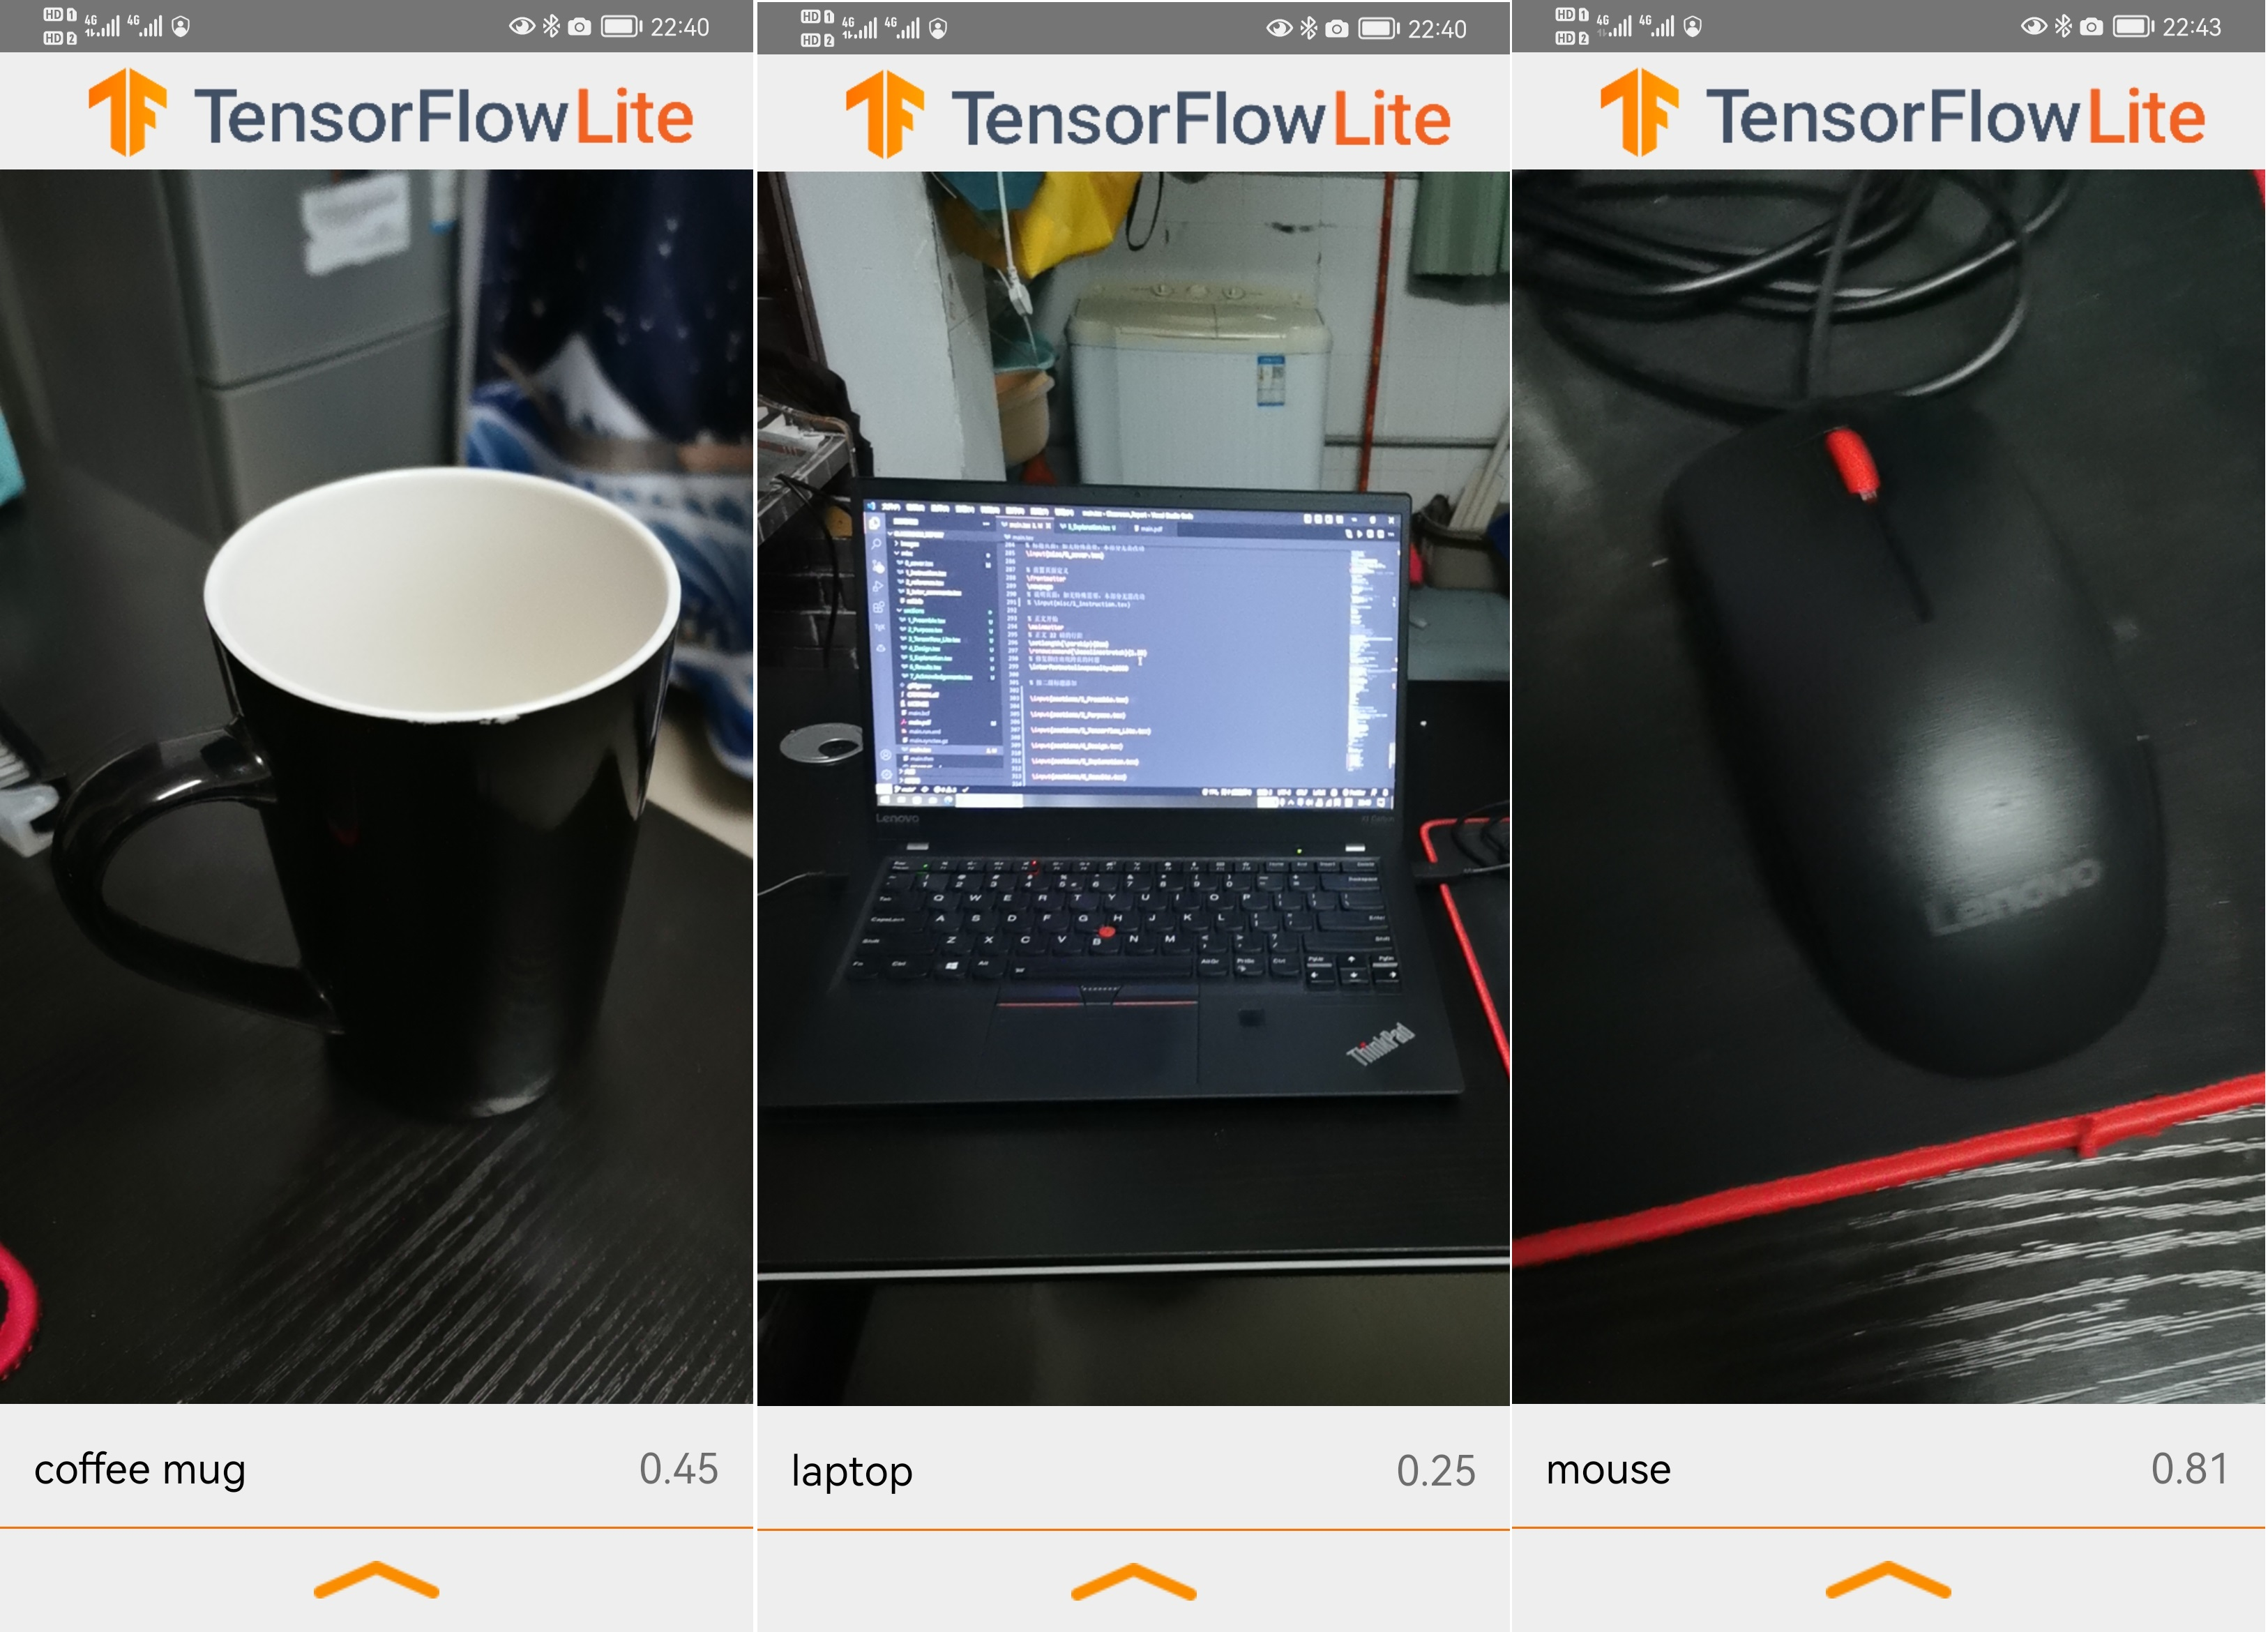
\includegraphics[width=0.8\textwidth]{images/1.eps}
  \caption{实际效果}
\end{figure}

\section{致谢}
最终要感谢在整个课程设计过程中帮助过我所有人。首先,也是最主要感谢的是我的指导老师,尚璇老师。
在整个过程中她给了我很大的帮助,在课设计划制定时,她首先确定了我的题目大方向,但是同时又帮我详细分析
使我有了明确的目标,尚璇老师丰富的教学经验和严谨的治学之道,潜移默化的影响了我的学习学涯。在课程设计
的过程中,尚璇老师的全力支持、严格要求和悉心指导,使我的课程设计得以完成。其次也非常感谢帮助过我的室友
和同学,在我遇到问题时帮助我走出困境,这次做课设的经历也会使我终身受益,我感受到做课程设计,是真正的自
己学习的过程和研究的过程,希望这次的经历能让我在以后学习中激励我继续进步。

% 参考文献  
% %%
% NCHU Bachelor Proposal Report Template
%
% 南昌航空大学毕业设计开题报告 (参考文献) —— 使用 XeLaTeX 编译
%
% Copyright 2023 Arnold Chow
%
% The Current Maintainer of this work is Arnold Chow.
%
% Compile with: xelatex -> biber -> xelatex -> xelatex
%
% 如无特殊需要,本页面无需更改

\section{参考文献}

% 设置参考文献字号为 5 号
\renewcommand*{\bibfont}{\zihao{5}}
% 设置参考文献各个项目之间的垂直距离为 0
\setlength{\bibitemsep}{0ex}
\setlength{\bibnamesep}{0ex}
\setlength{\bibinitsep}{0ex}
% 设置单倍行距
\renewcommand{\baselinestretch}{1.2}
% 设置参考文献顺序标签 `[1]` 与文献内容 `作者. 文献标题...` 的间距
\setlength{\biblabelsep}{0.5mm}
% 设置参考文献后文缩进为 0(与 Word 模板保持一致)
\renewcommand{\itemcmd}{
  \addvspace{\bibitemsep} % 恢复 \bibitemsep 的作用
  \mkgbnumlabel{\printfield{labelnumber}}
  \hspace{\biblabelsep}}

% 删除默认的「参考文献 / Reference」标题,使用上面定义的 section 标题
\printbibliography[heading=none]
% 导师意见
% %%
% NCHU Bachelor Proposal Report Template
%
% 南昌航空大学毕业设计开题报告(指导老师意见)—— 使用 XeLaTeX 编译
%
% Copyright 2023 Arnold Chow
%
% The Current Maintainer of this work is Arnold Chow.
%
% Compile with: xelatex -> biber -> xelatex -> xelatex

\section{指导教师意见}

\textcolor{blue}{指导教师提出具体意见,并表明是否同意毕业设计(论文)开题。}
\textcolor{blue}{此部分需手写并签名,请在阅读后删除该段文字。}


\end{document}
